\documentclass[sigconf,review]{acmart}

%%
%% \BibTeX command to typeset BibTeX logo in the docs
\AtBeginDocument{%
  \providecommand\BibTeX{{%
    \normalfont B\kern-0.5em{\scshape i\kern-0.25em b}\kern-0.8em\TeX}}}

\setcopyright{acmcopyright}
\copyrightyear{2019}
\acmYear{2019}
\acmDOI{10.1145/xxxxxxx.yyyyyyy}

\acmConference[SC19]
{The International Conference for High Performance Computing, Networking, Storage, and Analysis}
{November 17--22, 2019}{Denver, CO, USA}

\begin{document}

\title{What Deploying MFA Taught Us About Changing Infrastructure}

\author{Abe Singer}
\affiliation{National Energy Research Scientific Computing Center (NERSC)}
\email{abe@lbl.gov}

\author{Shane Canon}
\affiliation{National Energy Research Scientific Computing Center (NERSC)}
\email{scanon@lbl.gov}

\author{Rebecca Hartman-Baker}
\affiliation{National Energy Research Scientific Computing Center (NERSC)}
\email{rjhartmanbaker@lbl.gov}

\author{Kelly L.\ Rowland}
\orcid{https://orcid.org/0000-0001-5147-0051}
\affiliation{National Energy Research Scientific Computing Center (NERSC)}
\email{kellyrowland@lbl.gov}

\author{David Skinner}
\affiliation{National Energy Research Scientific Computing Center (NERSC)}
\email{deskinner@lbl.gov}

\author{Craig Lant}
\affiliation{National Energy Research Scientific Computing Center (NERSC)}
\email{clant@lbl.gov}

\begin{abstract}

NERSC is not the first organization to implement multi-factor authentication
(MFA) for its users, and we had seen multiple talks by other supercomputing
facilities who had deployed MFA.  But as we planned and deployed our MFA
implementation, we found that nobody had talked about the more interesting and
difficult challenges, which were largely social rather technical. Our MFA
deployment was a success, but, more importantly, much of what we learned could
apply to any infrastructure change. Additionally, we developed the sshproxy
service, a key piece of infrastructure technology that lessens user and staff
burden and has made our MFA implementation more amenable to scientific
workflows.

\end{abstract}

\begin{CCSXML}
<ccs2012>
<concept>
<concept_id>10002978.10003029.10003032</concept_id>
<concept_desc>Security and privacy~Social aspects of security and privacy</concept_desc>
<concept_significance>500</concept_significance>
</concept>
<concept>
<concept_id>10002978.10003029.10011703</concept_id>
<concept_desc>Security and privacy~Usability in security and privacy</concept_desc>
<concept_significance>500</concept_significance>
</concept>
<concept>
<concept_id>10002944.10011122.10002947</concept_id>
<concept_desc>General and reference~General conference proceedings</concept_desc>
<concept_significance>100</concept_significance>
</concept>
</ccs2012>
\end{CCSXML}

\ccsdesc[500]{Security and privacy~Social aspects of security and privacy}
\ccsdesc[500]{Security and privacy~Usability in security and privacy}
\ccsdesc[100]{General and reference~General conference proceedings}

\keywords{multi-factor authentication, MFA, infrastructure}

\maketitle

\section{Introduction}
\label{intro}

The National Energy Research Scientific Computing Center (NERSC) is the primary
scientific computing facility for the Office of Science in the U.S. Department
of Energy, located at Lawrence Berkeley National Laboratory (LBNL). More than
7,000 scientists use NERSC to perform basic scientific
research across a wide range of disciplines, including climate modeling,
research into new materials, simulations of the early universe, analysis of data
from high energy physics experiments, investigations of protein structure, and a
host of other scientific endeavors. In 2018, NERSC introduced multi-factor
authentication (MFA) to users; use of MFA at NERSC became mandatory in early
2019. In this paper, we describe the constraints under which we chose to
implement MFA, the challenges encountered in the process, solutions we found to
those challenges, and other technical points of interest generated along the
way. Detailing this transition may be useful to other facilities where planned
changes in digital infrastructure must be implemented while minimizing impact on
user productivity.

The most interesting part of implementing and deploying MFA was not the
technical aspects (though we did develop some innovative technology), but the
social factor of getting users enrolled and using MFA. Not unlike the transition
from Telnet to SSH or from one batch system to another, this digital transition
is complicated by the scale and diversity of our user workloads, software and
services, as well as user needs for workflow automation. The MFA transition at
NERSC is useful as a point of reference in similar large-scale changes in
scientific computing infrastructures.

As we were not under a formal mandate for MFA, we were not constrained by
prescriptive standards, so we had the freedom to implement our solution in a
manner that best supports our users' scientific needs. In the remainder of this
paper, we describe the goals of the MFA project at NERSC, detail specific
requirements imposed on the project by the communities supported at NERSC,
present technical and social solutions that were developed through the course of
the project, and conclude with a summary.

\section{Goal}
\label{goal}

The overall goal of the work described in this paper was to enhance security in
how users authenticate to NERSC systems and services by requiring multiple
factors while minimizing the impact on users' ability to get science done. Doing
so in a scalable and supportable way across a diverse scientific workload
presents challenges of a technical and social nature. MFA is not new to most of
the NERSC user community in their daily lives, but its role in scientific
workflows comes with requirements in need of unique solutions described below.

\section{Requirements}
\label{reqs}

NERSC's unique position as the primary scientific computing facility for the
Office of Science means that NERSC's diverse user base performs a wide variety
of different computational workflows using NERSC resources. This includes
anything from simple SSH sessions where a user submits jobs by hand to
elaborate, multistep, automated workflows. Because of this, first and foremost
special consideration needed to be given to minimize the impact of the new MFA
requirement across the spectrum of use cases. NERSC has maintained a reputation
with its users for being a productive computing facility where the cybersecurity
requirements are largely hidden from the users, so we could not afford to create
a cumbersome process that would not accommodate automation in these special
workflows.

% Shane added this to respond to comment #3.
Unlike many other HPC sites, NERSC does not require users to hop through a
gateway system or connect to a VPN to access resources.  This direct access model 
is critical for many complex workflows and users have applauded this ease of access in the past.
Because of this direct access model, NERSC could not simply implement MFA on some
perimeter system instead it needed to be integrated throughout the center.

Another important factor in the technologies we chose to use in the MFA project
was flexibility. Any particular authentication technology could eventually have
fundamental vulnerabilities discovered, or weaknesses in the underlying
cryptographic algorithms (e.g., MD5, DES, etc. \cite{xie2013fast,
diffie1977special}). Thus, it should be possible to change out the
authentication technology, should vulnerabilities be discovered, without having
to rebuild our entire authentication infrastructure; being too tightly wedded to
any particular solution could leave us at the risk of having a vulnerable system
that we could not change.

Further, a token is supposed to be ``something that you have''. As such, it is
also something that you can lose. Soft-tokens, in particular, are vulnerable to
loss of or destruction of data (e.g., reformatting) on the device upon which
they are stored. Thus we wanted to allow users to have multiple active tokens so
that they were less impacted should they e.g., lose their phone, keys, laptop.

We faced an additional complexity of supporting multiple platforms. Unlike many
commercial services, our users do not log into a single application, nor are the
applications all web services.  We had to be able to support MFA over multiple
command-line and web services, including SSH, Shibboleth/SAML-based
authentication, custom web services, data transfer services, and NERSC RESTful
API services.  Being able to integrate MFA with single-sign-on technologies
(e.g., Shibboleth, Kerberos) was also desirable.

Any additional steps users have to take to enroll and use our systems are an
increase in complexity.  With increased complexity come increased support calls.
We wanted to avoid users overloading our support staff just because they
couldn't get MFA to work.  Additionally, we wanted to keep the overall support
costs down, for both staff as well as equipment, licenses, etc.

Finally, as one of the largest American HPC centers, NERSC is a high-profile
target for hackers worldwide. NERSC systems are continuously under attack and
NERSC already devotes extensive efforts to security. We did not want to entrust
third-party vendors with secrets such as OTP seeds or depend on a third party
for a trusted path to authentication for concerns that this would increase the
risk of third-party hacks compromising our systems.


\section{Solution and Approach}
\label{solns}

\subsection{Design of MFA Implementation}
\label{design}

When designing the MFA implementation, NERSC carefully considered measures to
increase the ease of use and minimize impact on users. Of particular interest
were means that could also minimize additional burden to NERSC staff.

\subsubsection{Early Implementation Design and User Testing}
\label{early}

As NERSC embarked on the process of implementing and deploying MFA for its
users, we first evaluated different options and performed user testing with
early prototypes.  NERSC reviewed the solutions at other large HPC centers and
spoke to staff from those centers to hear about their experiences.  NERSC also
spoke to users who had experience with using these other facilities.  This
helped us identify a few candidate solutions to consider.  Some of these
solutions were then tested by NERSC staff and evaluated on ease of use, ease of
integration, cost, and support overhead.

NERSC conducted a series of user testing exercises prior to finalizing the
implementation choices.  NERSC had approximately 60 users, consisting of both
staff and user volunteers, work through the process of registering a token and
using MFA in their regular routine.  This prototype was not fully integrated
with the account management system so didn't cover the full user experience, but
it gave us feedback that both helped us solidify the technology choices and
helped us identify typical issues encountered by users.  It also helped in
identifying workflows or use cases that were particularly problematic with MFA.
For example, we realized that some web logins used the same authentication
password to authenticate to multiple backend services, which would break under
MFA.

\subsubsection{User Experience Implementation Design}
\label{user}

Among the design goals of the MFA infrastructure was to make the user experience
as positive as possible and to minimize the load on support staff. To this end,
instead of requiring a hard token, NERSC chose free, software-based, one-time
password authenticators \cite{m2011totp} that users can download and install
themselves. This method is based on an open standard and is implemented by
multiple clients supported on a variety of platforms.  NERSC added features to
NIM, the NERSC identity management system, to allow users to provision their
authenticator. Thus users were able to install and configure MFA for their
account without an incremental cost to support staff time.

Most NERSC users have access to a smartphone, so the primary authenticator NERSC
selected for users is Google Authenticator \cite{gauth}, which can be installed
on most smartphones. Some users were unable to use a smartphone in the secure
environment of their workspace, or had a physical disability that prevented them
from using a smartphone in this manner. For these users, NERSC added support for
the Authy free authenticator \cite{authy}, which is available for Windows and
MacOS and also as a Google Chrome browser plug-in. The majority of users were
able to avail themselves of at least one of these options, but some chose other
options such as OnePass or Firefox plugins without NERSC support.

The majority of users set up an authentication token on their smartphone. A
typical consumer changes devices at least every couple of years, potentially
resulting in the user no longer being able to access NERSC resources. Without an
easy way for users to manage their authentication tokens, including a way to
recover after losing access to a phone or accidentally removing an active token,
users might be unable to work and would require extensive staff assistance. To
address circumstances in which a user loses access to all of their active
tokens, for whatever reason, NERSC developed a means for users to completely
remove all tokens from their account, then log in (without MFA) to NIM to set up
a new token.

In addition, NERSC wanted to make it possible for users whose tokens were not
immediately available to not be stuck and unable to work. For this purpose,
NERSC developed the capability within NIM for users to provision back-up
one-time passwords that a user could print and store in a safe place (e.g.,
wallet, locked drawer) to be used in the event of an emergency.

\subsubsection{Infrastructure Design}
\label{infra}

Figure \ref{mfa-diagram} shows a diagram of the MFA system at NERSC. Because an
MFA system is inherently more complex and potentially more fragile than
conventional single-password authentication, another design goal of the MFA
infrastructure was to ensure that users would not be impacted by authentication
failures due to maintenance or outages on the infrastructure itself. NERSC
operational staff built in redundancy, monitoring, and emergency controls to
mitigate this risk. First, the MFA infrastructure was built with a redundant
``shared-nothing'' design, enabling components to fail or be taken offline for
maintenance non-disruptively. Then, a complete suite of real-time checks were
added to NERSC's center-wide monitoring framework that continuously exercise the
MFA backend, performing authentication on frequent intervals and producing
alerts for Operations to dispatch to staff. As a last resort, the system was
designed with a ``kill switch'' capability that can be quickly activated by
Operations to temporarily deactivate the token authentication subsystem during a
loss of service. The redundancy, monitoring, and ``kill switch'' features of the
MFA infrastructure have all been used since launch to prevent, detect, and
respond to events that would have otherwise impacted users.

The core component of NERSC's MFA design is LinOTP. LinOTP is an open-source,
one-time password authentication server \cite{linotp} with a variety of features
that were well-aligned with NERSC's requirements.  LinOTP supports numerous
simultaneous  authentication methods, providing us with flexibility both in
options we were able to provide to our users, plus the ability to make changes
should a vulnerability be discovered in the method in use.  The software also
supports token provisioning and management, and an API for integrating those
features into existing infrastructure. Those features greatly reduced the effort
required for building the token infrastructure. As an added bonus, we were able
to leverage an existing LinOTP server run by the central IT department at LBNL.

NERSC was concerned that the external LinOTP server could create a potential
risk of disruption in service if there were issues with the LinOTP service or
connectivity issues.  To address this, NERSC developed an intermediate service,
OTPProxy, that sits between the clients and the LinOTP service.  This service
performs the LDAP authentication portion of MFA and then sends the one-time
password portion to the LinOTP service.  If the proxy is set in a ``fail-open''
mode and detects an error in the response, such as a connection error, it can
ignore the OTP portion and still permit the login.  This approach also helps
prevent cases where the user gets locked out of their account because of too
many failed attempts due to an issue in the OTP server.  This also provides a
single place in which we can temporarily disable the OTP check without having to
push out any changes to the clients.  NERSC has used this feature when the
LinOTP service has scheduled maintenance.  The users continue to authenticate
with the password plus one-time password, but are unaware that only the password
is being checked.  The prompt and user action is the same during the failure event.
This is advantageous for the user as they do not need to change their behavior.
The OTPProxy service is not currently openly released since it is fairly specialized
to our enviorrnment, but can be opened if there is interest.

\begin{figure*}[h!]
  \centering
  \includegraphics[width=\textwidth]{nersc-mfa.png}
  \caption{NERSC MFA system architecture.}
  \Description{NERSC MFA system architecture.}
  \label{mfa-diagram}
\end{figure*}

Another infrastructure design goal was to minimize the impact of MFA on users'
ability to conduct their research, particularly for users with complex workflows
that may require data transfer into or out of NERSC. MFA by its nature impedes
automated workflows, as it requires a user to enter a new password with each
connection. While the MFA policy allows for exemptions to the requirement in
cases where MFA would have a significant impact on a user's scientific work,
NERSC wanted to minimize the number of users who had MFA exemptions. A key NERSC
innovation, sshproxy, described in detail in Section \ref{proxy}, was
instrumental to achieving this goal. sshproxy allows users to use MFA to obtain
time-limited SSH keys that can be used with automated workflows. NERSC sets the
time limits based on the needs of the particular user or project, with a default
limit of one day.

As the implementation became usable, initial testing was conducted on small
groups of NERSC staff, followed by voluntary testing by friendly user teams, and
finally extending to a system-wide deployment. During this process NERSC was
able to refine the implementation based on user feedback. For example, in
addition to the option of scanning a QR code, we added support for manually
typing the shared seed into an authentication app.

\subsection{Automation and Operations}
\label{auto}

\subsubsection{sshproxy}
\label{proxy}

As noted above in Section \ref{goal}, a key concern in the move to MFA was
minimizing the impact to users and ensuring that automated workflows continued
to function. A number of projects rely on NERSC to provide automated analysis of
data coming from various instruments and detectors.  Many of these use cases are
tied to other user facilities that have their own set of users and metrics, and
changes in NERSC's policies can impact these facilities.  Many of these
automated use cases were already using SSH as the underlying method to transfer
data and trigger the execution of analysis pipelines.  Clearly, requiring a user
to enter a one-time password for each of these operations was not feasible.
Additionally, many users will log into NERSC system many times a day and
requiring them to enter their one-time password each time impacts their
productivity.  NERSC required a solution that would allow users and robot
accounts to access systems via SSH but with strict controls on the lifetime of
the access and other limits.  NERSC developed a RESTful-based service called
sshproxy to generate and maintain SSH keys to help meet these requirements. 
This allows a user to generate a long-lived key that can be used in automated workflow 
for an extended period of time (potentially up to a year).  The user only needs to authenticate
with their password and token when they generate the key.  The
sshproxy architecture is shown in Figure \ref{sshproxy-diagram}.
Workflows that already relied on SSH were able to easily convert over to using
the long-lived keys without any changes to their process or workflows.

\begin{figure}[h!]
  \centering
  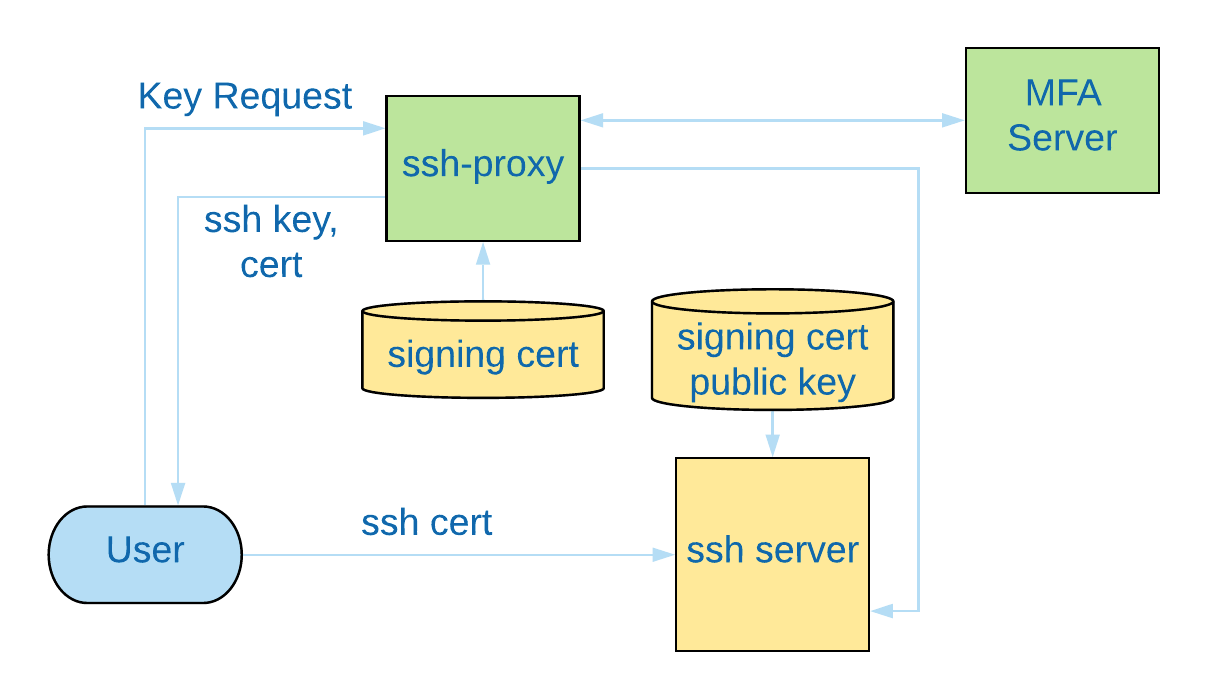
\includegraphics[width=\columnwidth]{sshproxy.png}
  \caption{sshproxy architecture.}
  \Description{sshproxy architecture.}
  \label{sshproxy-diagram}
\end{figure}

The sshproxy service works by allowing the user to authenticate using MFA to the
service and generate an SSH private key and certificate \cite{habets2011} that
can then be used to connect to NERSC systems using standard SSH clients.  This
request is done with a simple shell script that the user can run on their remote
system.  The generated key has a default lifetime of 24 hours.  This lifetime is
typically sufficient for most daily interactive work.  For use cases that
require longer lifetimes such as automated workflows, users can request the
ability to generate extended life-time keys that can span from weeks to a year.
In general, these longer lifetime keys require stricter limits on where the keys
can be used.  For example, the keys would be limited to the IP addresses of the
instrument system in a given scientific workflow.

Since sshproxy greatly enhances the usability of the MFA system, it was
important that it could be used on various OS platforms and SSH clients.  The
service can generate keys that can be used by OpenSSH clients, SSH client
libraries and many Windows-based SSH clients such as PuTTY.  It has been tested
with Windows, OSX, and Linux.  While the service can generate signed
certificates that are honored by NERSC systems, the service also supports a
fallback mechanism for older clients that may not support these certificates.
This fallback mechanism makes use of OpenSSH's \textit{AuthorizedKeysCommand}
which allows the server to run an executable to get the list of valid authorized
keys.  In our case, this script makes a request to the sshproxy service to get
the list of currently active keys for the user.  The service can also generate
keys to access ``collaboration accounts'' which are shared accounts primarily
used by large collaborations and projects.  In this case, the user authenticates
using their personal account and MFA credentials, but the generated key maps to
the collaboration account.

% respond to comment #2
An alternative to sshproxy is to use OpenSSH's built-in control master functionality \cite{openssh}.
This allows multiple sessions to reuse a connection.  The main disadvantage of this
approach is once the control connection is severed (e.g. a network issue, login node
reboot, etc), the session must be reauthenticated.  So this is less useful for automated
workflows or even laptop access where the network connection may change.

The sshproxy service has become a key component of the overall NERSC MFA
architecture.  The software has been approved for public release and NERSC is
planning to make it public in the near future, hopefully by the end of 2019.

\begin{figure*}[ht!]
  \centering
  \includegraphics[width=\textwidth]{uptake.png}
  \caption{User enrollment in MFA in 2018, from initial rollout to mandatory requirement.}
  \Description{User enrollment in MFA in 2018, from initial rollout to mandatory requirement.}
  \label{uptake}
\end{figure*}

\subsubsection{Host-based Authentication}
\label{host}

Another important usability component is making sure NERSC users are not
required to re-authenticate once they are inside the NERSC domain (e.g., SSH
from one NERSC system to another).  NERSC implemented host-based access to
address this.  However, one challenge in using SSH host-based authentication is
managing and propagating keys.  NERSC utilized another feature of SSH
certificates \cite{redhat2019} which allows the target system to be configured
with a signing authority that can be used to validate a signed host key.  NERSC
maintains a well-protected signing host that is used to generate certificates
for the various NERSC systems.  The client systems are then configured to
present this certificate as part of the host-based authentication exchange.  The
key advantage of this approach is that if new hosts are added or host keys need
to be regenerated, the new keys can be signed and configured on the client
system and no additional changes are required on the target systems.

\subsubsection{Exemptions and Edge Cases}
\label{edge}

While the combination of the sshproxy service and host-based authentication has
addressed most use cases, some examples have emerged that still require further
work.  For example, one project has a series of remote sensing devices that are
extremely difficult to access and make updates to.  NERSC has an MFA exemption
process to ensure these projects can continue to function and NERSC is working
to further enhance the sshproxy tool to address these edge cases.

\subsection{Social Aspects}
\label{social}

With a point-in-time deadline for users to switch to using MFA, NERSC was
concerned about the impact on support staff should the thousands of NERSC users
wait until the deadline and then enroll in MFA all at once. To minimize this
impact, NERSC set a goal of having 1,000 existing users enrolled by the end of
December 2018. This goal not only served to reduce the number of users enrolling
at once, but to help NERSC identify and correct any issues with the enrollment
process ahead of the deadline.

Figure \ref{uptake} shows the number of NERSC users enrolled in MFA over 2018;
key points spurring MFA uptake are annotated on the plot. To meet and eventually
exceed our goal of 1,000 users enrolled in MFA by January 2019, we took a multi-
pronged approach to user communications which included personalized messages,
targeted engagements, and open office hours.

NERSC conducted an extensive communications campaign along several fronts. The
User Engagement Group (UEG) developed thorough, clear documentation for users on
how to enroll and use MFA. The campaign to inform users of the plan kicked off
in August 2018 with an announcement by the NERSC Director that MFA would become
mandatory in the new allocation year. Over the following months department heads
sent memos to users encouraging enrollment and testifying to the ease of use,
and NERSC published profiles on the NERSC website of users who had successfully
transitioned to using MFA, which included a discussion of their research and the
minimal impact of MFA on their workflows. In November and December 2018, UEG
reached out to projects with high usage and low MFA enrollment, encouraging them
to enroll before the deadline and offering help if there were any questions. UEG
included reminders and announcements of new features in the NERSC weekly
newsletter, and MFA was the topic for three of the weekly podcasts. Finally, UEG
held several rounds of virtual ``office hours'' where support staff spent the
day online in a video conference room, and users could dial in and ask
questions.

Emails from NERSC management resulted in upticks in adoption of MFA. As the
deadline approached, many users embraced the inevitable and signed up. Most
users were able to transition to MFA without NERSC assistance, but we helped
more than 100 users during the office hours in the final days before and
immediately following the deadline.

\section{Summary}
\label{summary}

NERSC successfully deployed a new MFA system over a 12-month period, converting
the majority of its users to using MFA for authentication by the beginning of
the new allocation year. Through the process of implementing and deploying MFA,
NERSC staff took home a variety of lessons from the project. First, the social
factors of the technologies are just as important as their technical merits. To
implement a change of this magnitude, high-quality, frequent communication with
users is crucial. Second, technology choices that minimize the additional load
on staff and users alike are essential. Finally, implementing a new technology
should minimize changes in users' daily routines. If the burden of a new
requirement is too high, users will look for ways to circumvent it. Thus, we
introduced the NERSC sshproxy service lessen user and staff burden and better
enable scientific computing workflows.

\bibliographystyle{ACM-Reference-Format}
\bibliography{hpcsyspros19}

\appendix

\section{Email Text Sent to Users}

\end{document}
